%!TEX root = ../main.tex

\section{Aim of the experiment}
The low temperature properties of different solids are determined in the experiment. Especially the electrical resistance of metals, semiconductors and superconductors. We expect a phase shift for the superconductor which requires special consideration. 

\section{Electrical resistance of metals}


A simple description with the Drude model can be used for metals. The electrons are accelerated in an electric field and scattered at the atomic cores after a mean free path. It follows for the electrical conductivity:
\begin{equation}
    \sigma = \frac{ne^2\tau}{m_e}
\end{equation}
where n is the charge carrier density, $\tau$ is the mean free time, and e is the elementary charge. The temperature dependent conductivity follows from the mean free time $\tau$. This is due to the scattering of electrons by phonons and impurities in the lattice. The resistivity is given by $\sigma =\frac{1}{\rho}$ to Matthiessen's rule:
\begin{equation}
    \rho = \rho_{ph}(T) + \rho_{im}
\end{equation}
The scattering at impurities is independent of temperature and is reflected in a constant residual resistance. The following temperature dependencies apply to phonon scattering:
\begin{itemize}
    \item For high temperatures ( $T > \Theta_D$, with $\Theta_D$ Debye temperature).
    \begin{equation}
        \rho_{ph} \propto T
    \end{equation}
   \item For low temperatures ($T<\Theta_D$) 
    \begin{equation}
        \rho_{ph} \propto T^5
    \end{equation}
    
\end{itemize}
Where for high temperatures, according to Grüneisen-Bornelius, one can determine the Debye temperature with:
\begin{equation}
	\label{eq:HT}
    R_T = 1,17\frac{R(\Theta_D)}{\Theta_D} T-0,17\cdot R(\Theta_D)
\end{equation}


\section{Semiconductors}
Semiconductors are very different from normal conductors like metals. For $T \rightarrow 0$ the valence band is completely filled and the conduction band is empty. One can distinguish between intrinsic and extrinsic semiconductors.


\subsection{Intrinsic semiconductor}


Since neither a full valence band nor an empty conduction band contributes to charge transport, the electrons have to overcome an energy gap $E_{gap}$ to the next band. This is done by thermal excitation, which is obviously temperature dependent. Thus for the electrical conductivity follows:
\begin{equation}
    \sigma_{tot} = \sigma_e+\sigma_h =n_ie(\mu_e+\mu_h)
\end{equation}
where $n_i$ corresponds to the electron / hole density and $\mu$ to the corresponding mobility. In the end, the following equation is obtained:
\begin{equation}
    \sigma_i = C_i \exp{\left (-\frac{E_{gap}}{2k_BT}\right)}
\end{equation}
Thus, the electrical conductivity approaches the constant $C_i$ asymptotically.


\subsection{Extrinsic semiconductor}
By doping a semiconductor, its conductivity can be strongly increased. In this process impurities of the neighboring main group are added. These atoms either donate electrons (donors) or accept electrons (acceptors) and produce a n/p doped semiconductor. Sub-energy levels are created in the band gap which can be excited more easily. This results in a complicated temperature profile with $\sigma = en\mu$.
\begin{figure}
    \centering
    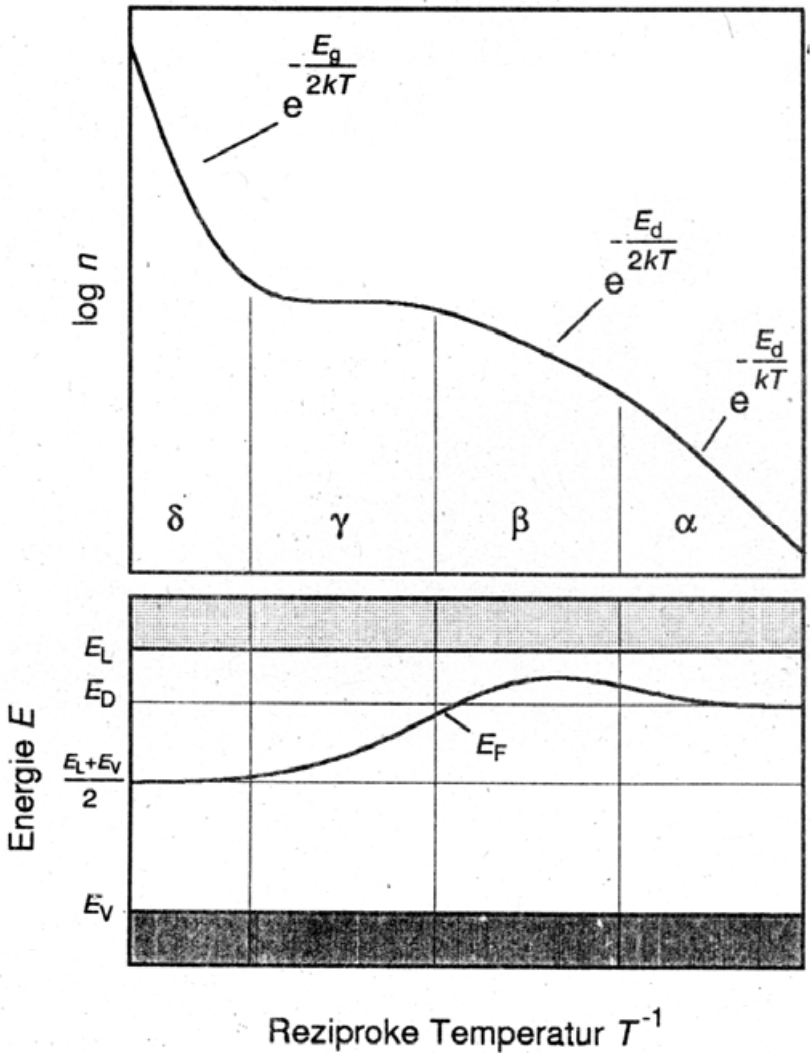
\includegraphics[width=0.5\textwidth]{./fig/exhl.png}
    \caption{Temperature dependent charge carrier concentration in extrinsic semiconductors.}
    \label{fig:exhl}
\end{figure}


\section{Superconductors}



Unlike metals and semiconductors, a superconductor has a critical temperature $T_c$. Below this temperature the electrical resistance disappears and the superconductor behaves like an ideal conductor. Due to the Meissner-Ochsenfeld effect, the superconductor also behaves like a diamagnet ($\chi = -1$). One can distinguish between metallic and kermaic superconductors. Metallic superconductors usually have lower critical temperatures. 
These phenomena can be described by the BCS theory. Two electrons form a Copper pair with spin 1. So they behave like bosons, do not obey the Pauli principle like single electrons and have no total momentum.
\begin{align*}
    (\Vec{k} \uparrow , -\Vec{k} \downarrow )
\end{align*}
This behavior is explained via the polarization of the atomic lattice by the first electron and the resulting attraction of the second electron. The phonons are the exchange particles of this exchange interaction. 
The Copper pairs all occupy the same quantum mechanical state at low temperatures and are therefore firmly correlated. If now an external electric field is applied, all copper pairs get the same momentum. However, the individual Cooper pairs cannot exchange momentum with the lattice because they are all in the same state and not all electrons can be scattered simultaneously. This effect describes nothing else than resistanceless charge transport through the lattice. 
However, the stability is limited by the binding energy of the pair correlation of the Cooper pairs. If the momentum of the Cooper pairs increases by the electric field and thus their energy exceeds the binding energy, the interaction with the lattice starts again. Thus, there is a critical momentum (equivalent to current density) above which the superconductor becomes a normal conductor.

\subsection{Superconductor in magnetic field}
From the critical current density implied above, a critical magnetic field follows immediately. This behavior is described by the Meissner-Ochsenfeld effect. Here, the external magnetic field induces continuous currents at the surface of the superconductor and the external magnetic field is forced out of the inside . However, a small London penetration depth $\lambda$ exists. One can now distinguish between two types of superconductors:
\begin{itemize}
    \item superconductors 1st kind show the Meissner effect up to a critical field $B_{c,th}$.
    \item Superconductors 2nd kind show the Meissner effect up to $B_{c1}$ and then enter the Shubnikov phase up to a field $B_{c2}$.
\end{itemize}

\begin{figure}
    \centering
    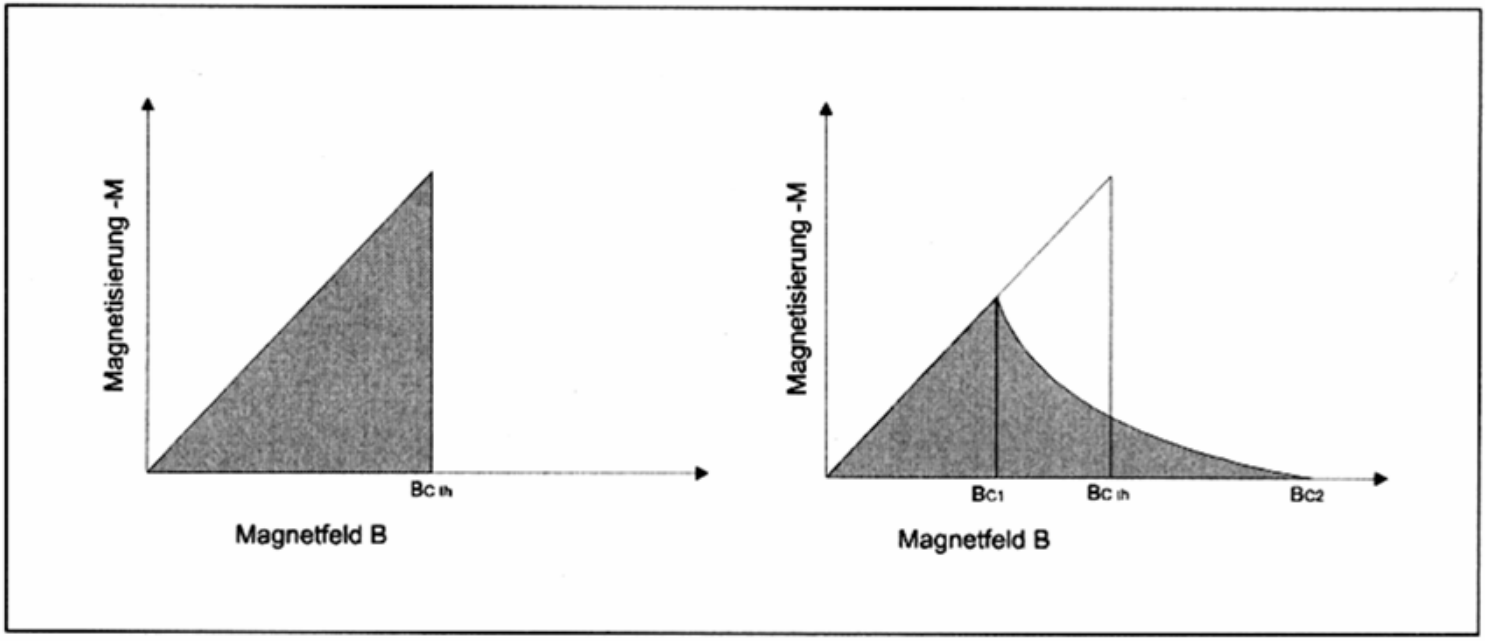
\includegraphics[width=0.8\textwidth]{./fig/super.png}
    \caption{Magnetization curve of superconductors 1st kind (left) and 2nd kind (right)}.
    \label{fig:super}
\end{figure}


\subsection{Ginsburg-Landau Theory (GLAG)}
Considering the problem as a phase transition, one can define an order parameter $\phi$ near the critical temperature. In our case, this describes the Cooper pair density and accordingly vanishes in the disordered phase for $T>T_c$. If we now develop the free energy density as powers of the order parameter in thermodynamic equilibrium, it becomes minimal. Thus, all other thermodynamic quantities can be derived such as the critical magnetic field $B_{c2}$, the Ginzburg-Landau coherence length $\xi_{GL}$ and the London penetration depth $\lambda$.
\begin{equation}
    \lambda(T) = \lambda(0) \left( 1-\left( \frac{T}{T_C }\right )^4\right )^{-1/2} 
\end{equation}

For the upper critical field $B_{c2}$, it follows:
\begin{equation}
    B_{c2}(T) = \frac{\Phi_0}{2\pi\xi_{GL}^2(T) }
\end{equation}
with flux quantum $\Phi_0=\frac{h}{2e}$ and GL coherence length $\xi_{GL}$:
\begin{equation}
    \xi_{GL}(T) = \frac{\xi_{GL}(0)}{\sqrt{1-T/T_c}}
\end{equation}
When T = 0, it follows:
\begin{equation}
    \xi_{GL}(0)=\left[\frac{- \Phi_0}{2 \pi T_c \frac{dB_{c2}}{dT}|_{T_c}} \right ]
\end{equation}
and the mean free path $l$ for niobium as normal conductor is given by:
\begin{equation}
    \xi_{GL}(0) = \sqrt{\SI{39}{nm}\cdot l}
\end{equation}


